\chapter{基于LTE的人群密度预测算法}
\label{chap:algorithm}

基于第二章提到的理论知识,本章节我们将针对基于LTE的人群密度监控算法进行详细的讨论。

根据第二章的理论,我们可以得到一下结论:

\begin{enumerate}
    \item 基于LTE的定位技术对于67\%的用户设备定位精度可以达到40m,并且响应时间能够控制在1s以内。
    \item 使用E-CellID技术和OTDOA技术无需用户安装第三方软件,即可实现在用户移动的过程之中进行定位。
    \item 使用LTE技术定位,在不混合GPS定位技术的前提之下,周围环境对定位精度影响较小。适用于人口密度较大的特大城市的场景。
\end{enumerate}
通过上述的结论,我们通过LTE可以方便的收集用户的定位数据,但是定位精度有限。在本章节的第一部分中我们将会详细的介绍位置特征的收集方式。

在收集到用户设备的位置信息后,我们会分别使单拟合、使用相邻区域特征的GBDT算法和自动编码器提取特征的GBDT算法等算法进行预测。简单的线性拟合算法是通过拟合某个小区内人群总数的变化,通过趋势来预测未来的人口数量。我们分别使用相邻区域人群个数和相邻区域信息熵两种特征加入到GBDT算法当中,分别对各个小区的人口趋势进行预测,最后我们对这两种算法进行对比,分析各自的优劣。

通过上述分析,人群密度预测算法的过程如下。

对于拟合算法犹如下流程:
\begin{enumerate}
    \item 通过收集基站数据,收集用户设备的位置信息。
    \item 通过收集到的用户设备位置信息,计算每个小区的人群密度
    \item 分别对每个小区内的人群密度进行拟合,通过拟合方程预测未来每个小区的人群密度。
\end{enumerate}

对于GBDT预测算法流程如下:
\begin{enumerate}
    \item 收集用户设备的位置信息。
    \item 计算每个小区内的人群密度。
    \item 根据相邻小区和小区内的人群密度抽取特征。
    \item 将得到的特征使用GBDT机器学习模型进行训练。
    \item 使用得到的训练模型对未来的人群密度进行预测。
\end{enumerate}
算法的流程图,如图\ref{fig:algo-flow}所示。

\begin{figure}[!htp]
    \centering
    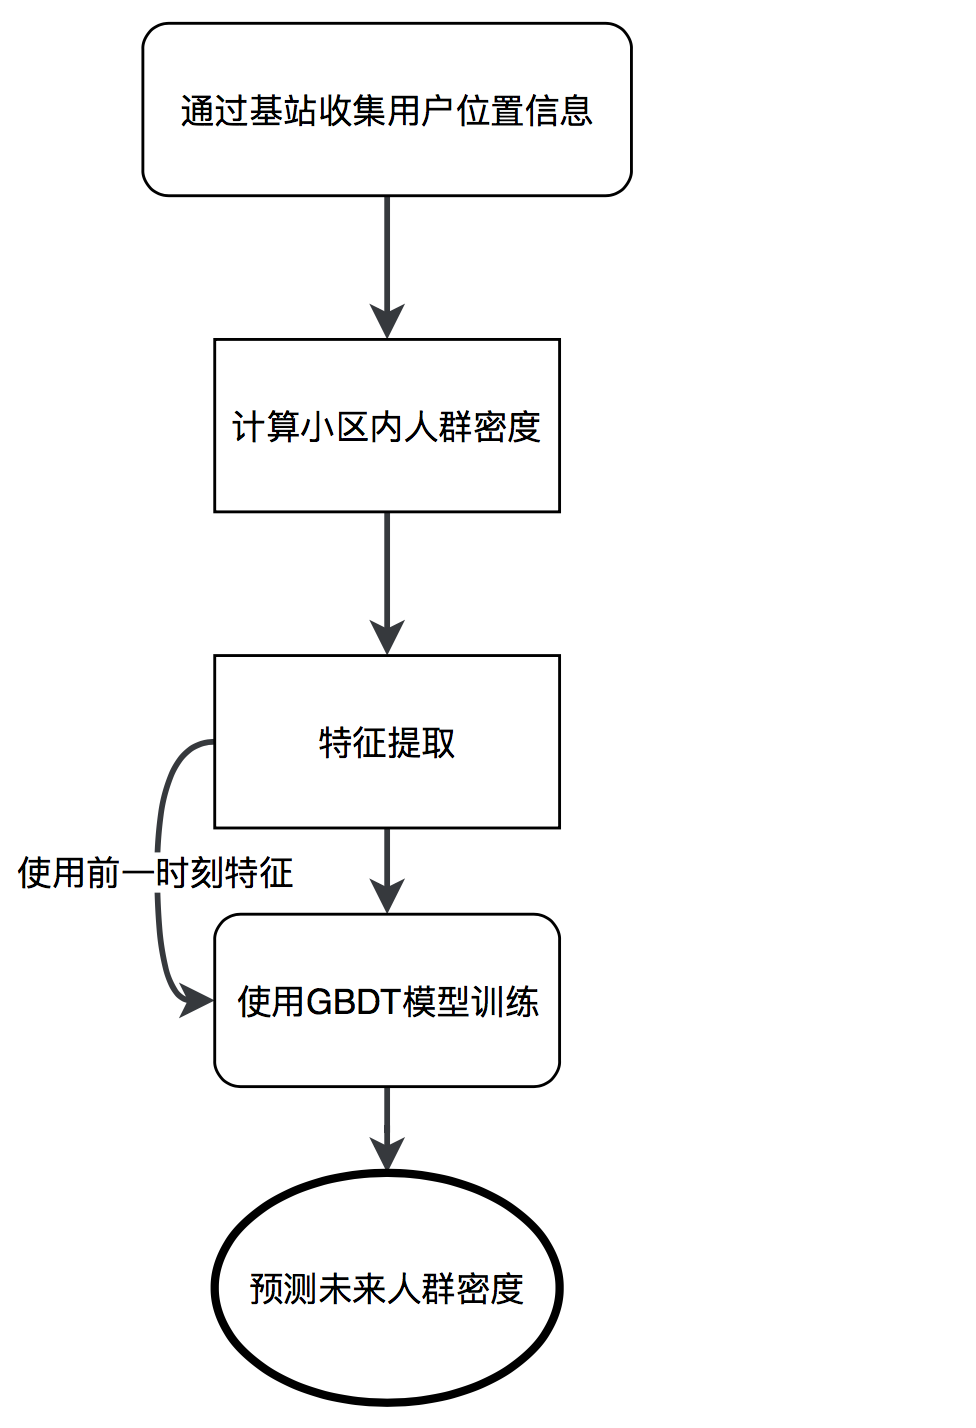
\includegraphics[width=0.8\textwidth]{chap3/algo-flow}
    \bicaption[fig:algo-flow]{算法流程图}{算法流程图}{Fig.}{Algorithm Flowchart}
\end{figure}

\section{位置特征收集}

在当下基于LTE的定位协议经过多年的发展已经逐步稳定,已经能够充分满足定位精度和响应时间的需求。两种新的协议已经被标准化来实现LTE定位:LTE定位协议(英文:Long-term evolution Positioning Protocol,缩写:LPP)\cite{lpp}和LTE定位协议附件(英文:Long-term evolution Positioning Protocol Annex,缩写:LPPa)\cite{lppa}。 LPP是定位服务服务器和定位服务目标设备之间的点对点协议,用于定位目标设备。两个协议中已经规定了以下事务:传输数据,辅助数据传送过程和位置信息传送过程。可以串联或并联使用任何上述类型的多个LPP过程。 LTE定位系统的方框图如\ref{fig:ran-sys}所示:

\begin{figure}[!htp]
    \centering
    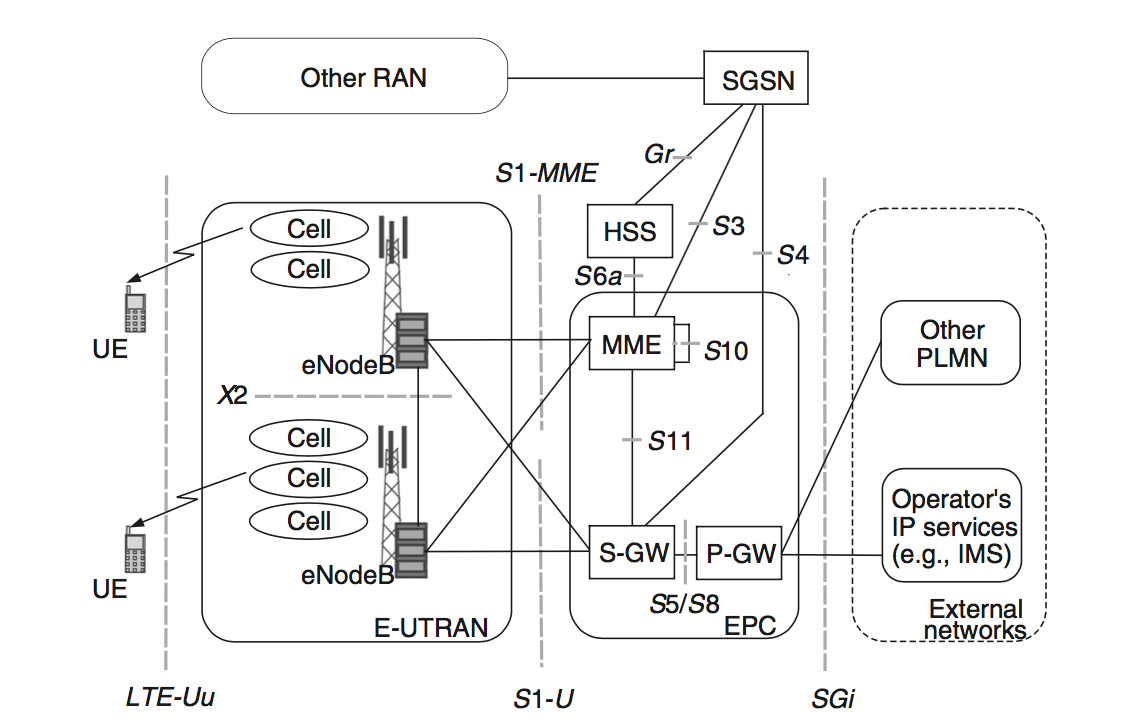
\includegraphics[width=0.8\textwidth]{chap3/ran-sys}
    \bicaption[fig:ran-sys]{LTE系统框架}{LTE系统框架}{Fig.}{LTE System Architecture}
\end{figure}
其中每个\textit{cell}是在LTE系统中含有ID的最小实体,例如Cell ID、用户设备等。每个eNodeB和每个\textit{cell}含有全局唯一的ID,每个eNodeB可以服务多个cell。E-UTRAN与UE之通过在LTE-Uu接口进行无线电通信。在E-UTRAN中,eNodeB可以通过逻辑X2接口互连,逻辑X2接口主要用于移动性和一些无线电资源管理,E-UTRAN通过逻辑接口S1连接到EPC。LTE E-UTRAN接口和协议结构被组织成两个逻辑独立的plane:\textbf{control plane}和\textbf{user plane}。control plane主要用于应用协议,在涉及不同网络节点的若干接口上操作(例如,S1-AP\cite{s1ap}是通过S1接口发送的应用协议,而X2-AP\cite{x2ap}是通过X2接口发送的),以及用于传输也就是传递应用协议消息的信令。其中control plane中的顶层协议是在用户设备和EPC之间操作的非接入层(英文:nonaccess stratum,缩写:NAS)。它使用LTE-Uu接口上的无线资源控制(英文:radio resource control,缩写:RRC)协议和S1接口上的S1-AP协议作为传输协议,而user plane包括由用户平面隧道协议和传输的数据流构成。

对于Control Plane为了支持定位服务(LCS),control plane架构中必须存在至少两个功能节点:演进服务移动定位中心(英文:Evolved Serving Mobile Location Center,缩写:E-SMLC)用于控制定位移动设备所需的资源的协调和调度,以及移动网关定位中心(英文:Gateway Mobile Location Center,缩写:GMLC)用于控制位置数据的传递、用户授权、收费等。使用LTE定位协议进行用于定位相关信息传输。 LPP对移动管理实体(英文:Mobility Management Entity,缩写:MME)也是可见的,然后在使用LPPa在S1-MME和SLs接口上透传数据。control plane的LTE定位架构如图\ref{fig:cp}所示。其中MME接收到与特定LCS目标(例如用户设备)相关联的一些LCS的定位请求。然后,MME在LCS-AP位置请求消息中向LCS发送LCS请求。 E-SMLC处理LCS请求以执行目标用户设备的定位任务。E-SMLC然后将LCS的结果返回给MME。最终MME会将结果转发到请求节点。
\begin{figure}[!htp]
    \centering
    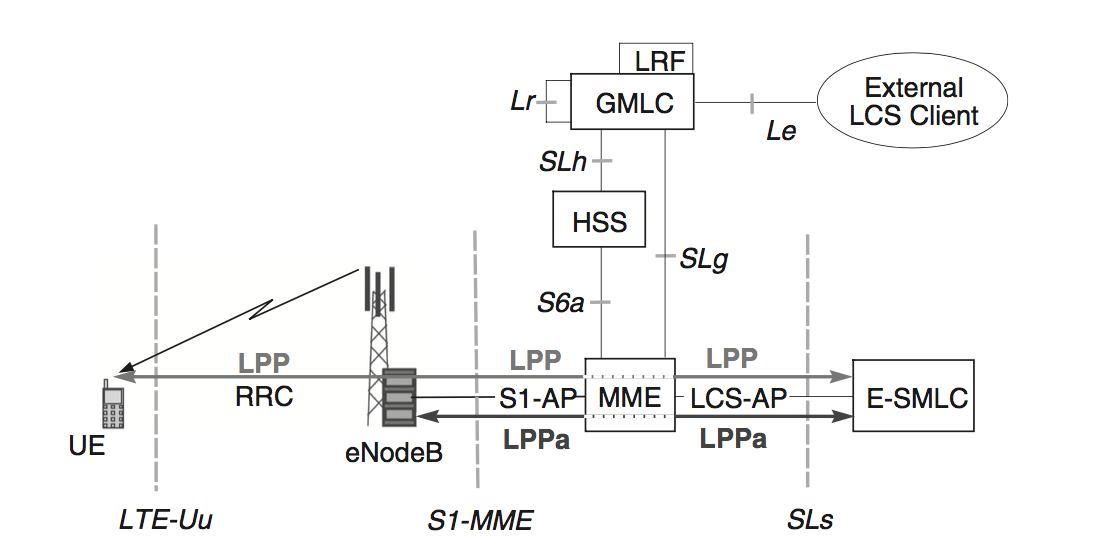
\includegraphics[width=0.8\textwidth]{chap3/control-plane}
    \bicaption[fig:cp]{Control Plane定位框架}{Control Plane定位框架}{Fig.}{Control Plane System Architecture}
\end{figure}

在收到这些信号并通过坐标变换之后,即可通过第二章中提到的定位技术对用户设备进行定位。在LTE定位规范中规定67 \%的设备精度要达到50m,而实际情况中定位精度与用户的信号强度、有无遮挡物、定位服务器负载有着很强的关系。

\section{数据处理}

由于LTE定位精度限制,我们不能将每个行人的精确位置带入到模型当中,我们只能得到行人的大致位置。于是在本文中将采取以下做法,将整个地图区域$A$按照50m为一个单位进行分解,也就是将地图分成网格状结构,于是对于任意一个行人$P_{i}$都可以根据定位得到的坐标$(x, y)$将其放置在地图上的某个方格$A_{m,n}$内。但是我们得到的行人位置并非正确的行人坐标(有着50m左右的误差),于是我们以采集到的行人$P_{i}$的坐标为圆心以25m为半径在地图上画圆,如图\ref{fig:circle}所示,那么我们可以通过每个方格内圆形覆盖的面积得到该行人$P_{i}$在四个方格内的概率,即我们将圆形在方格$A_{m,n}$内覆盖的面积$S_{i,m,n}$作为该行人在区域内的概率,在该时刻对于行人$P_{i}$在方格$A_{m,n}$有$S_{i,m,n}$个人,对地图上所有的人进行上述操作,我们可以得到每个区域中的行人个数,如式\ref{eq:pd}。

\begin{figure}[!htp]
    \centering
    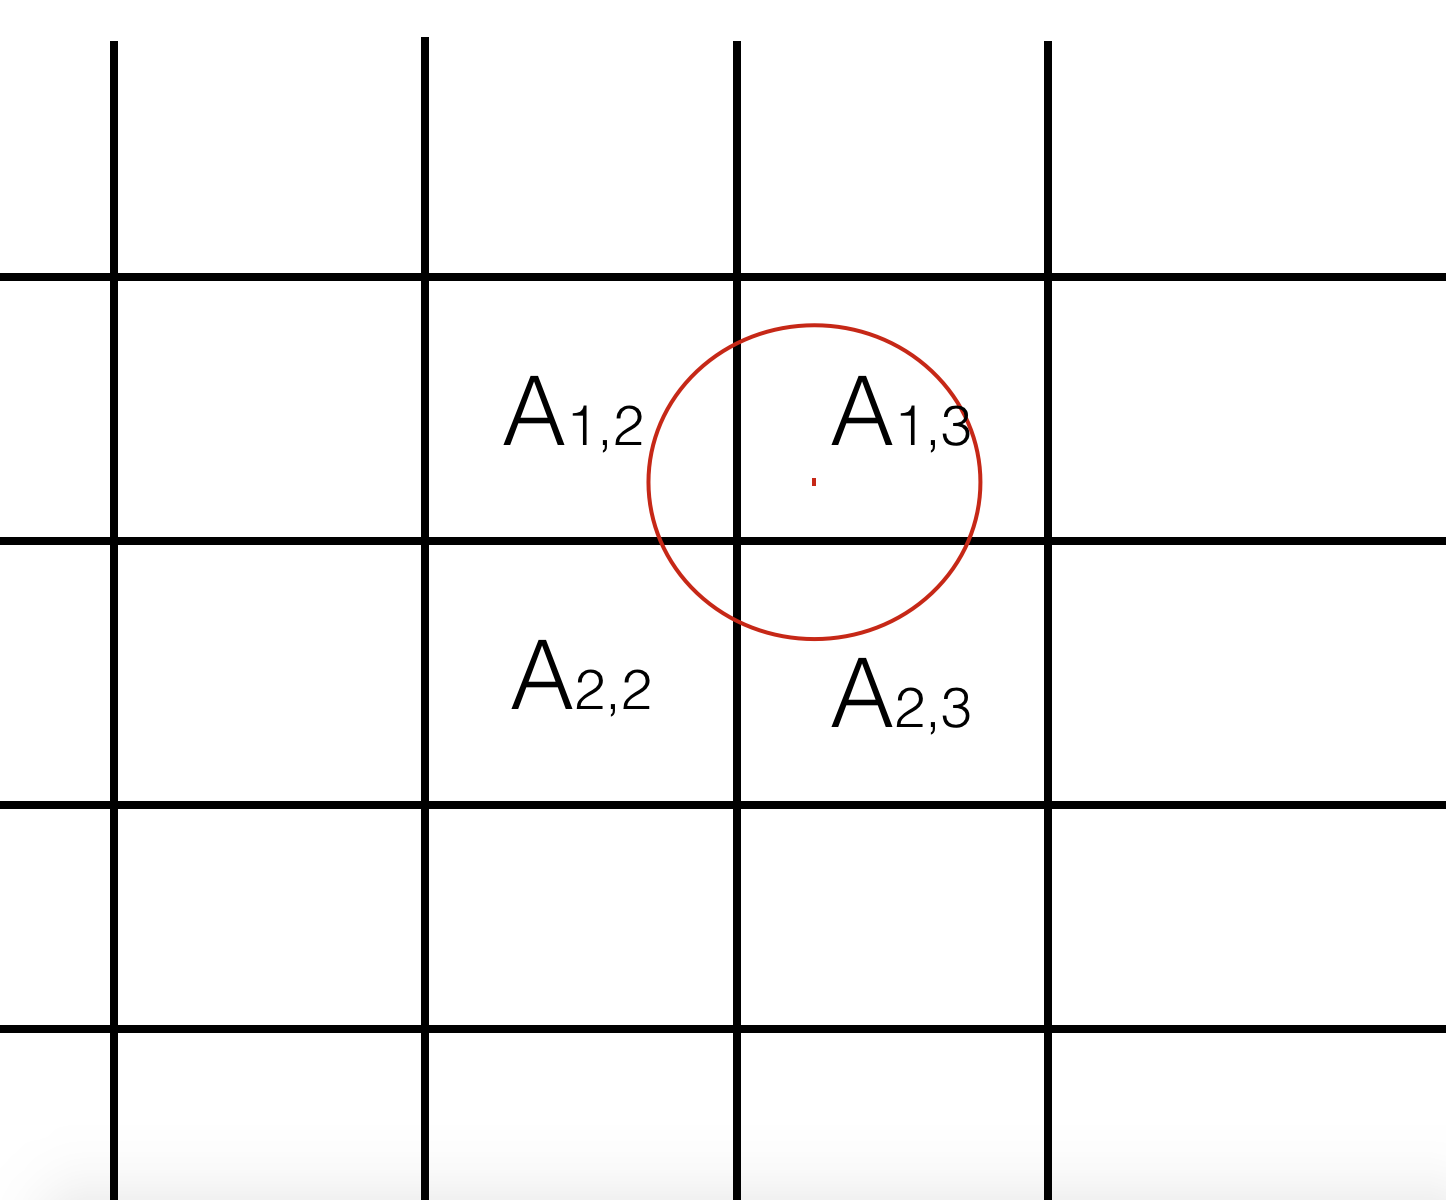
\includegraphics[width=0.6\textwidth]{chap3/circle}
    \bicaption[fig:circle]{行人在区域中分布}{行人在区域中分布}{Fig.}{Pedestrians Circle}
\end{figure}

\begin{figure}[!htp]
    \centering
    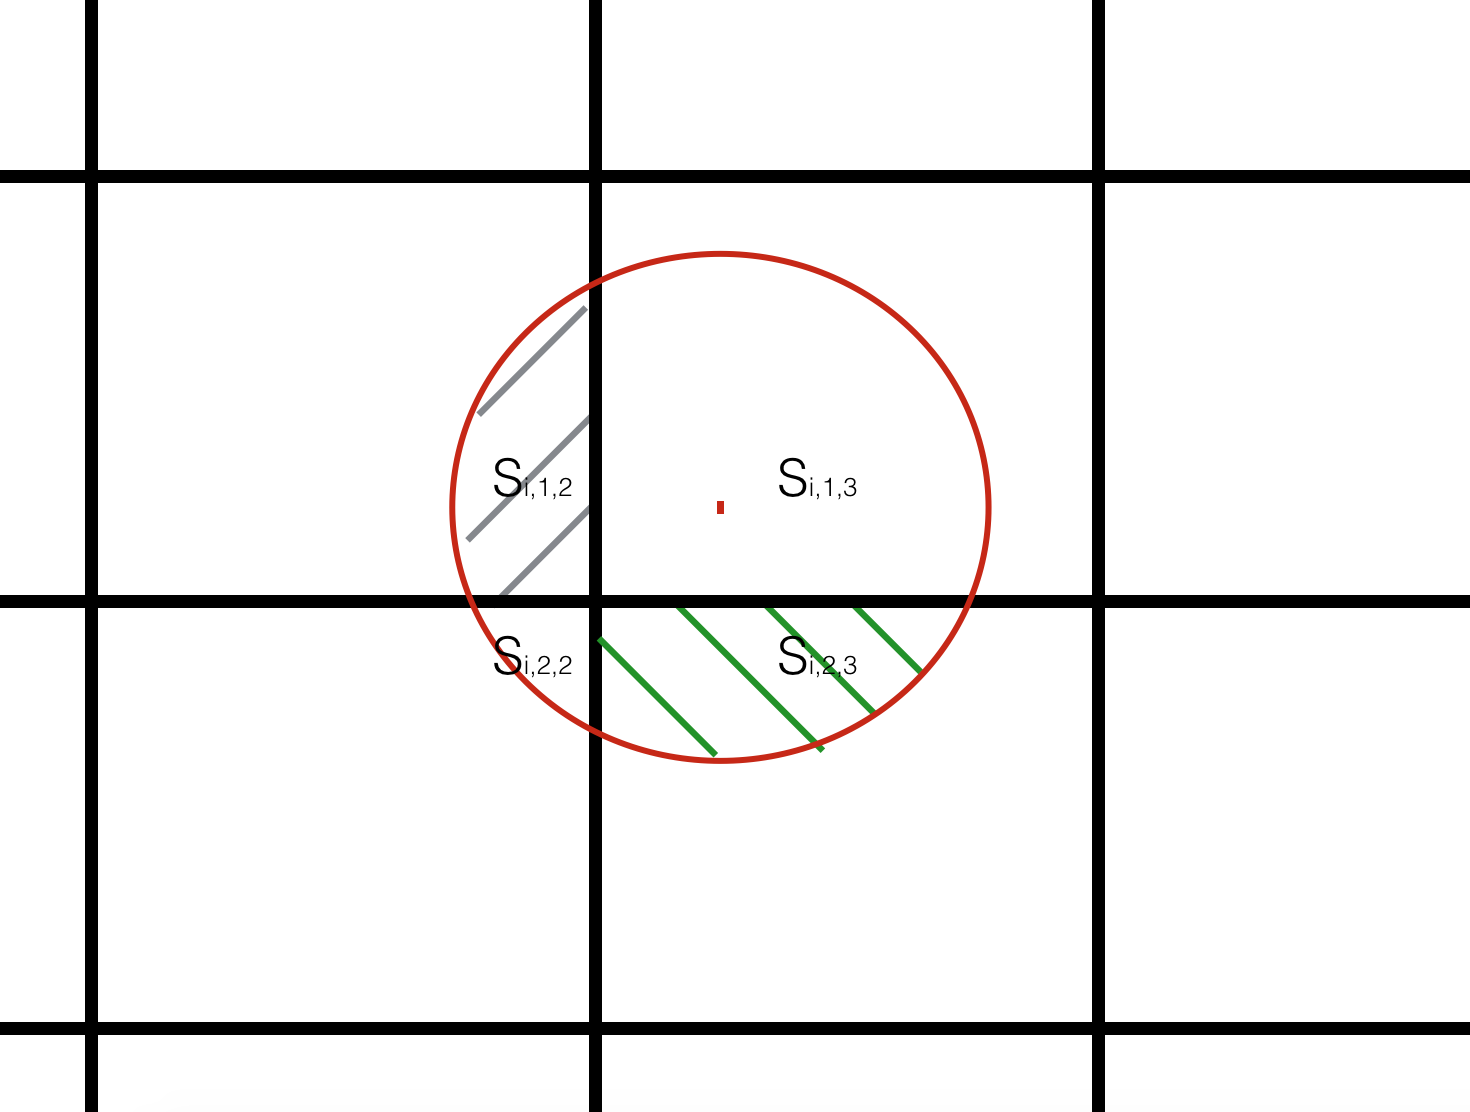
\includegraphics[width=0.6\textwidth]{chap3/circle2}
    \bicaption[fig:circle2]{行人分布概率}{行人分布概率}{Fig.}{Pedestrians Circle}
\end{figure}

\begin{equation}
    \label{eq:pd}
    D(m,n)=\sum_{i=1}^{N}S_{i,m,n}
\end{equation}
其中N代表行人综述,${D(m,n)}$即为区域$A_{m,n}$的人群密度。

算法流程如\ref{algo:group}

\begin{algorithm}
    \caption{LTE数据处理算法}
    \label{algo:group}
    \begin{algorithmic}[1]
    \For{$P = 1 \to N$}
        \State $x,y \gets Position(P_{i})$
        \State $S_{i,m,n} \gets Probability(x, y)$
    \EndFor
    \For{$m = 1 \to m_{max}, n = 1 \to n_{max}$}
        \State $D_{m,n} \gets \sum_{i=1}^{N}S_{i,m,n}$
    \EndFor
    \end{algorithmic}
    \State
    \Return $D_{m,n}, m=1,...,m_{max}, n=1,...,n_{max}$
\end{algorithm}
其中$Position(P_{i})$为获取行人$P_{i}$的位置信息,$Probability(x,y)$为通过坐标获取相交的方格的行人概率。

\section{基于回归的预测算法}

按照上一小节提到的算法将行人个数按照小方格进行划分之后,这一节的算法中我们分别对每个方格的数据进行拟合以达到预测未来人群密度的目的。本课题当中的问题可以描述为,已知在$1,2...T$时刻,我们分别知道小区内人群密度分别为$D_{1},D_{2},...,D_{T}$,要根据这些已知的数据预测$T+1,T+2,...T+m$时刻的人群密度。基于回归的预测算法当中我们可以认为未来$T+m$时刻的人群密度只与之前$T$时刻的数据有关,所以我们只要将前$T$时刻的数据通过现有的回归算法进行拟合,然后将$T+m$时刻这一变量代入其中即可得到$T+m$时刻的人群密度,达到我们的算法的目的。

在这里我们先要对比数学中常用的几种拟合算法包括线性回归、多项式回归、逐步回归等算法,找出最适合我们应用场景的拟合算法。

\begin{enumerate}
    \item \textbf{线性回归算法} \\
    线性回归算法是最知名而是最简单的回归模型,我们可以在平面直角坐标系当中建立时间和人群密度之间的关系。可以使用以下函数\ref{eq:linear}来从数学角度解释线性回归:
   
    \begin{equation}
        \label{eq:linear}
        y_i = \alpha + \beta x_i + \varepsilon_i.
    \end{equation}
   
    最终的目的是找到$y=\alpha +\beta x$使得对数据源来说最合适,线性拟合的过程就是找到合适的$\alpha$和$\beta$的过程。通常的办法是使用最小二乘法\ref{eq:linear2}
   
    \begin{equation} 
        \label{eq:linear2}
        ${\displaystyle {\text{找到最小的 }}\min _{\alpha ,\,\beta }Q(\alpha ,\beta ),\qquad {\text{使得 }}Q(\alpha ,\beta )=\sum _{i=1}^{n}\varepsilon _{i}^{\,2}=\sum _{i=1}^{n}(y_{i}-\alpha -\beta x_{i})^{2}\ }$
    \end{equation}
   
    \item \textbf{多项式回归} \\
    多项式回归是线性回归的一种推广形式,其中独立变量$x$和因变量$y$之间的关系被建模为$n$阶多项式。多项式回归拟合了$x$的值和相应的y的值之间的非线性关系,表示为$E(y | x)$,并用于描述非线性现象,多项式回归被认为是多元线性回归的特殊情况。
    可以使用以下函数\ref{eq:polynomial}来描述:
   
    \begin{equation}
        \label{eq:polynomial}
        y = a_0 + a_1 x + a_2 x^2 + a_3 x^3 + \cdots + a_n x^n + \varepsilon. 
    \end{equation}
   
    可以通过矩阵计算得到最佳的拟合参数\ref{eq:poly-solve}。
    
    \begin{eqnarray}
        \label{eq:poly-solve}
        \displaystyle {\begin{bmatrix}y_{1}\\y_{2}\\y_{3}\\\vdots \\y_{n}\end{bmatrix}}={\begin{bmatrix}1&x_{1}&x_{1}^{2}&\dots &x_{1}^{m}\\1&x_{2}&x_{2}^{2}&\dots &x_{2}^{m}\\1&x_{3}&x_{3}^{2}&\dots &x_{3}^{m}\\\vdots &\vdots &\vdots &&\vdots \\1&x_{n}&x_{n}^{2}&\dots &x_{n}^{m}\end{bmatrix}}{\begin{bmatrix}a_{0}\\a_{1}\\a_{2}\\\vdots \\a_{m}\end{bmatrix}}+{\begin{bmatrix}\varepsilon _{1}\\\varepsilon _{2}\\\varepsilon _{3}\\\vdots \\\varepsilon _{n}\end{bmatrix}}, \\
        \vec y = \mathbf{X} \vec a + \vec\varepsilon. \\
        \widehat{\vec a} = (\mathbf{X}^T \mathbf{X})^{-1}\; \mathbf{X}^T \vec y.
    \end{eqnarray}
   
    % \item \textbf{LASSO回归}  在统计和机器学习中,最小绝对收缩和选择算子(英文:least absolute shrinkage and selection operator,缩写LASSO)是一种回归分析方法,执行变量选择和正则化,以提高其生成的统计模型的预测准确性和可解释性。它是由Robert Tibshirani在1996年根据Leo Breiman的Nonnegative Garrote提出\cite{tibshirani1996regression}。Lasso最初是为最小二乘模型制定的,Lasso执行子集选择的能力依赖于约束的形式,并且具有多种解释,包括在几何,贝叶斯统计和凸分析方面。
    % 从数学角度解释有如下公式\ref{eq:lasso}:
    
    % \begin{eqnarray}
    %     \label{eq:lasso}
    %     \displaystyle \min _{\beta _{0},\beta }\left\{{\frac {1}{N}}\sum _{i=1}^{N}(y_{i}-\beta _{0}-x_{i}^{T}\beta )^{2}\right\}{\text{ 其中 }}\sum _{j=1}^{p}|\beta _{j}|\leq t. \\
    %     \displaystyle \min _{\beta _{0},\beta }\left\{{\frac {1}{N}}\left\|y-\beta _{0}-X\beta \right\|_{2}^{2}\right\}{\text{ 其中 }}\|\beta \|_{1}\leq t. \\
    %     \displaystyle \min _{\beta \in \mathbb {R} ^{p}}\left\{{\frac {1}{N}}\left\|y-X\beta \right\|_{2}^{2}+\lambda \|\beta \|_{1}\right\}
    % \end{eqnarray}
   
    % Lasso回归在惩罚方程中用的是绝对值,而不是平方。这就使得惩罚后的值可能会变成0。
\end{enumerate}

这里我们充分比较了几种回归算法,通过理论知识和第四章的实验我们不难发现简单的多项式拟合在回归算法中最适合于我们的应用场景。在这里我们忽略周围相邻的方格对当前方格的影响,这种算法的优势是易于理解、无需太多的统计学的相关知识,不考虑周围环境的影响能够简单快速的得到预期的结果,但是由于忽略了周围环境的影响会导致预测结果并不准确,非常容易出现过拟合的现象。为了解决这些问题我们将引入机器学习当中的GBDT算法,该算法广泛的应用到了机器学习当中的回归问题和拟合问题当中,对于本课题当中的场景,有着较好的适用性。

\section{基于机器学习的预测算法}

在这一小节当中我们将使用基于机器学习算法作为我们的预测模型,我们将分别使用监督学习的GBDT算法和无监督学习的自动编码器进行建模。

\subsection{GBDT算法}
正如上一章所介绍的基础知识我们不难发现再GBDT算法有如下特性。

\begin{enumerate}
    \item 通过决策树的剪枝算法,能够有效地防止过拟合,在预测中有更好的准确率。
    \item 每一步的残差都会放大分错的值得权重,从而尽快的得到更优的模型。
    \item 残差作为全局最优的绝对方向,这个特性加快了梯度下降的速度。
\end{enumerate}

在GBDT算法当中特征选择和参数选择会极大地影响最终预测的效果,特征充分考虑过了周围相邻的方格对当前方格的影响,与上一章的回归算法不同,GBDT算法是融合多个特征作为输入参数进行训练,将训练得到到的模型作为预测模型,将未来$T+m$时刻的特征输入进训练模型当中即可得到预测结果。下面我们将介绍如何将现有的数据作为输入进行训练,然后预测未来的数据。

与直接的拟合直接将$T+m$直接作为因变量进行回归相比GBDT算法需要选择若干特征进行训练,通过监督学习得到预测模型。我们将特征选择的过程进行如下描述。

我们不妨设在$t$时刻我们有特征$f_{t,1},f_{t,2},...,f_{t,r}$总共$r$个特征,其中$1 \leq t \leq T$,我们要预测$T+k$时刻的人群密度,其中我们要求$k \ll T$,那么我们将特征按照时间排序并且分别向上错开$k$个特征,即我们选择$t$时刻的特征为$f_{t-k,1},f_{t-k,2},...,f_{t-k,r}$,其中$1 \leq t \leq T$,这样我们相较于之前$T$组数据,变成了$T-k$组数据。然后剩下的$k$组数据,分别为$\{f_{T-k+1,1},f_{T-k+1,2},...,f_{T-k+1,r}\}$,$\{f_{T-k+2,1},f_{T-k+2,2},...,f_{T-k+2,r}\}$,...,$\{f_{T,1},f_{T,2},...,f_{T,r}\}$,我们分别将其作为$T+1, T+2, ..., T+k$时刻的数据。这样我们分别将得到$k$组预测的结果。如表\ref{tab:feature}所示。

\begin{table}[!hpb]
    \centering
    \bicaption[tab:feature]{特征列表}{特征列表}{Table}{Features List}
    \begin{tabular}{@{}cccc@{}} \toprule
        时间 & 特征 \\ \midrule
        k+1 & $f_{1,1},f_{1,2},...,f_{1,r}$ \\
        k+2 & $f_{2,1},f_{2,2},...,f_{2,r}$ \\
        ... & ... \\
        T & $f_{T-k+1,1},f_{T-k+1,2},...,f_{T-k+1,r}$ \\ 
        T+1 & $f_{T-k+2,1},f_{T-k+2,2},...,f_{T-k+2,r}$ \\
        T+k & $f_{T,1},f_{T,2},...,f_{T,r}$ \\ \bottomrule
    \end{tabular}
\end{table}

在得到预测结果之后,我们需要对预测结果的准确率进行评价,将预测结果和真实的人群密度进行比较,比较其均方根误差。不妨设我们总共有$N$个小区,并且我们分别对这$N$个小区的未来$k$个时刻进行了人群密度预测。我们将小区$i$的未来$j$时刻的预测结果$Y_{i,T+j}$和真实的结果$D_{i,T+j}$使用式\ref{eq:comp}进行比较得到误差$E_{i,T+j}$:

\begin{equation}
    \label{eq:comp}
    E_{i,T+j}=\frac{|Y_{i,T+j}-D_{i,T+j}|}{D_{i,T+j}}
\end{equation}
其中$1 \leq i \leq N$,$1 \leq j \leq k$。进一步的我们将同一个小区的预测误差使用均方根误差如式\ref{eq:rms}计算的到该小区的预测误差$E_i$。

\begin{equation}
    \label{eq:rms}
    E_i={\sqrt  {\sum _{{j=1}}^{k}E_{i,T+j}^{2} \over k}}={\sqrt  {E_{i,T+1}^{2}+E_{i,T+2}^{2}+\cdots +E_{i,T+k}^{2} \over k}}
\end{equation}

更进一步的,由于这个$N$个小区在我们看来是等价的,所以取这$N$个小区的预测误差的平均值即整个地图区域的误差\ref{eq:average}。

\begin{equation}
    \label{eq:average}
    E={\sum _{{i=1}}^{N}E_{i} \over N}
\end{equation}
以上的过程可以用算法\ref{algo:predict}表示,流程图如\ref{fig:predict}所示:

\begin{algorithm}
    \caption{人群预测算法}
    \label{algo:predict}
    \begin{algorithmic}[1]
    \State Initial Data
    \For{$i = 1 \to N$}
        \State $F_{i,j} \gets LTE\_location(i,j), j=1,2,...,T$
        \State $Train(F_{i,j}), j=1,2,...,T-k$
        \State $Y_i \gets Predict(F_{i,T+j}), j=1,2,...,k$
        \State $E_{i,T+j} \gets \frac{|Y_{i,T+j}-D_{i,T+j}|}{D_{i,T+j}}, j=1,2,...,k$
        \State $E_i \gets {\sqrt  {\sum _{{j=1}}^{k}E_{i,T+j}^{2} \over k}}$
    \EndFor
    \State $E \gets {\sum _{{i=1}}^{N}E_{i} \over N}$
    \State 
    \Return $E$
    \end{algorithmic}
\end{algorithm}

\begin{figure}[!htp]
    \centering
    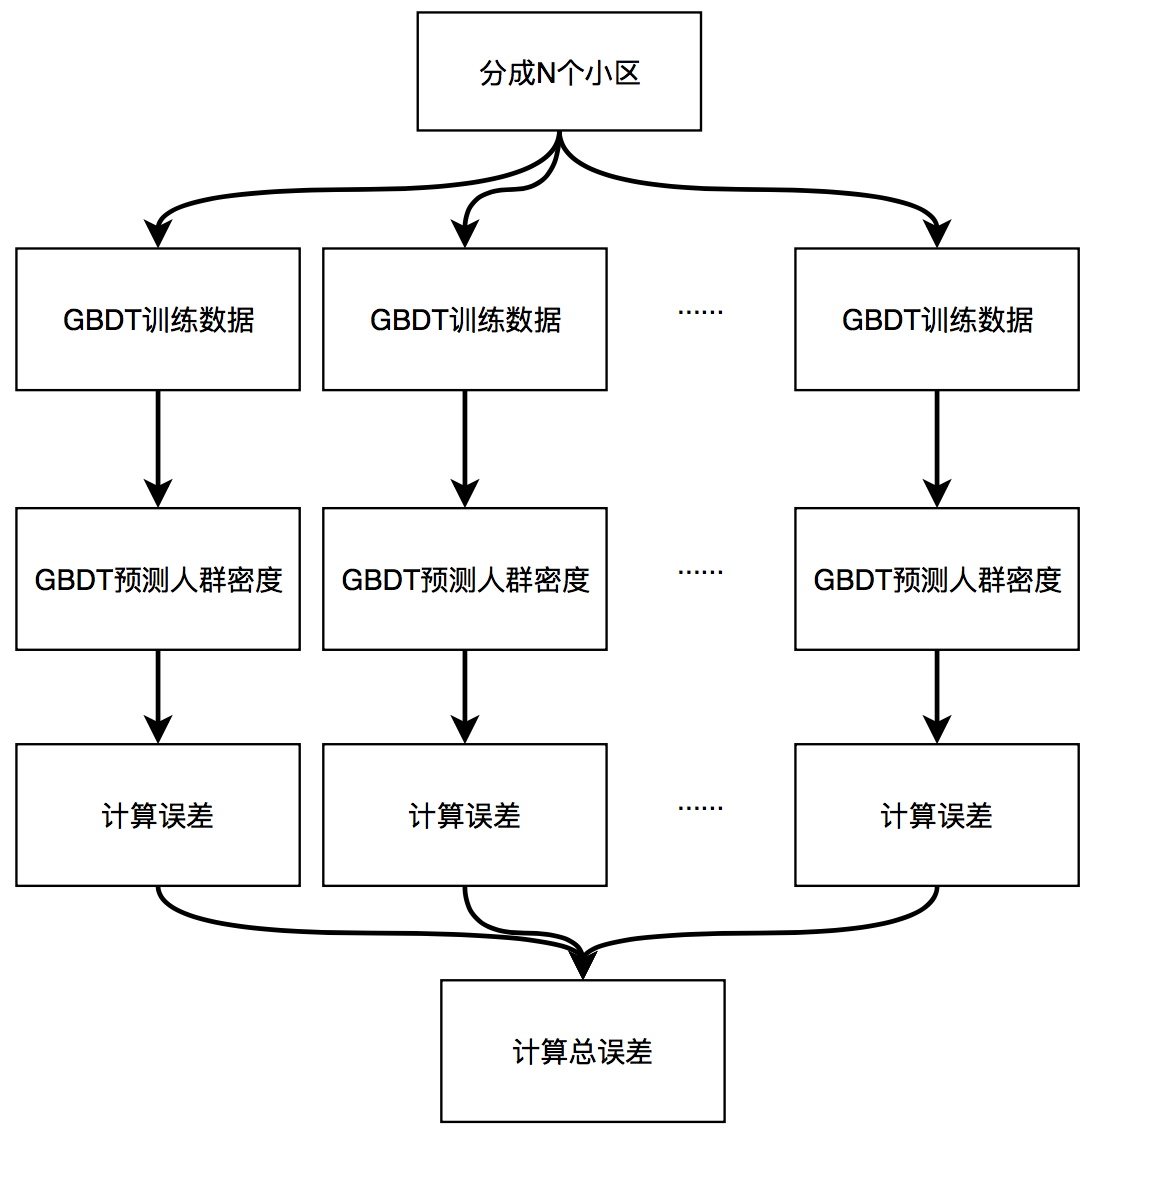
\includegraphics[width=0.8\textwidth]{chap3/predict}
    \bicaption[fig:predict]{预测算法流程}{预测算法流程}{Fig.}{Prediction Algorithm Flowchart}
\end{figure}

我们详细的介绍了算法的流程,提到算法中最重要的是特征选择,这一小节中我们将介绍特征提取的算法,基于相邻区域的特征。

这里我们将小区周围八个相邻小区的行人密度作为特征,这样在预测的过程中我们不仅将小区本身的人群密度考虑其中还将相邻小区之间的影响考虑进了模型当中,相邻小区特征的影响如图\ref{fig:neighbor}所示。

\begin{figure}[!htp]
    \centering
    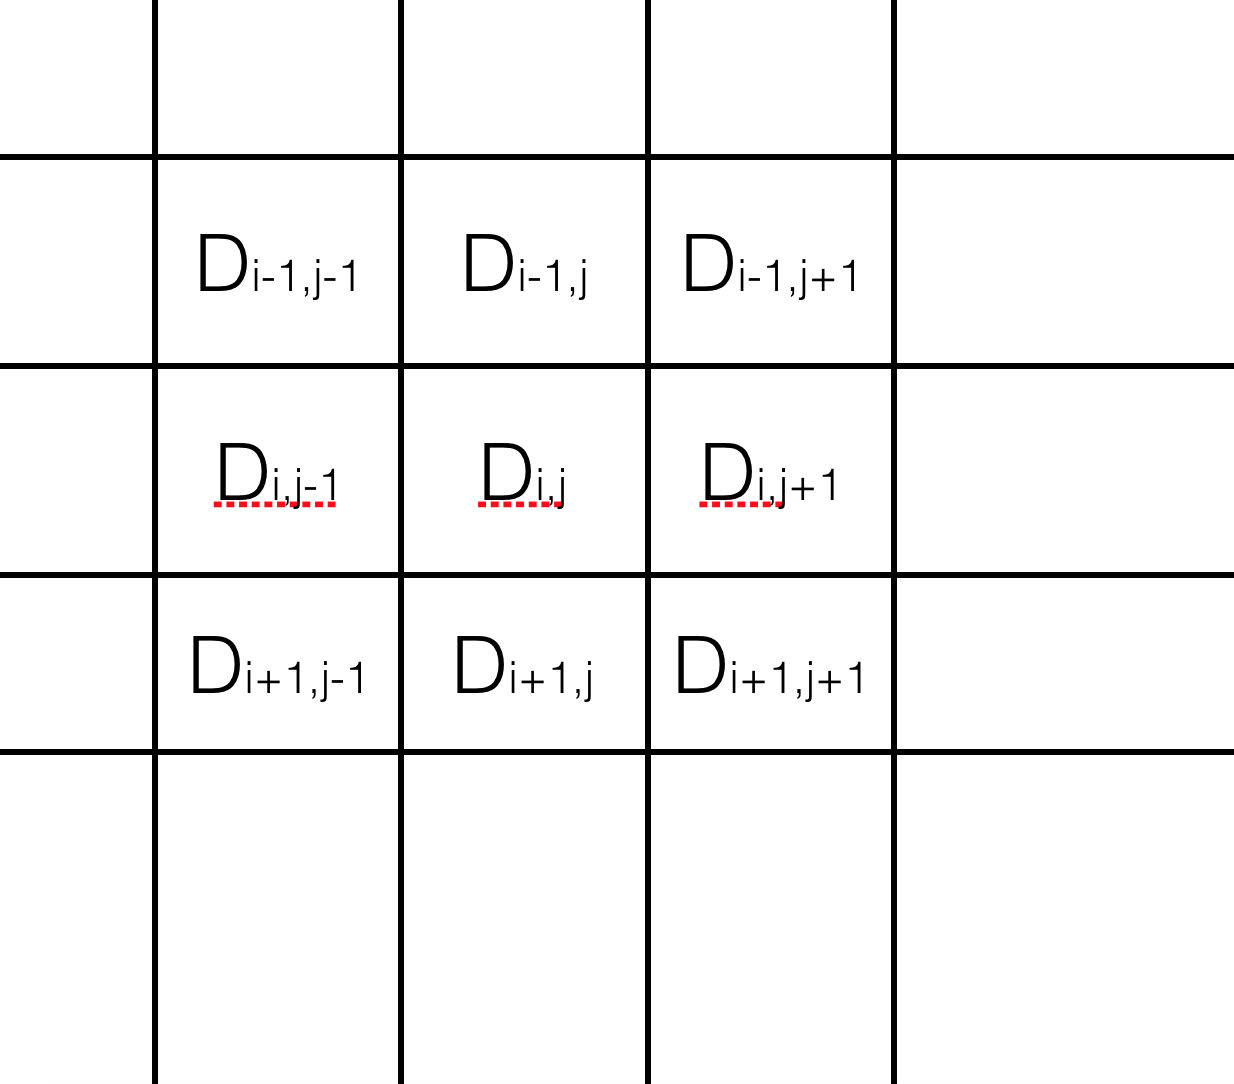
\includegraphics[width=0.6\textwidth]{chap3/neighbour}
    \bicaption[fig:neighbor]{相邻区域特征}{相邻区域特征}{Fig.}{Neighbor Feature}
\end{figure}

考虑小区$D_{i,j}$在我们的地图划分之中存在八个相邻的小区,分别为$D_{i-1,j-1}$,$D_{i-1,j}$,$D_{i-1,j+1}$,$D_{i,j-1}$,$D_{i,j+1}$,$D_{i+1,j-1}$,$D_{i+1,j}$,$D_{i+1,j+1}$这八个小区,我们将他们对应的人群密度作为特征,从而得到了9个特征,我们将这9个特征按照$D_{i,j}$,$D_{i-1,j-1}$,$D_{i-1,j}$,$D_{i-1,j+1}$,$D_{i,j-1}$,$D_{i,j+1}$,$D_{i+1,j-1}$,$D_{i+1,j}$,$D_{i+1,j+1}$的顺序进行排列使用GBDT算法进行有监督训练和预测。

\subsection{自动编码器算法}

本小节我们将使用无监督学习当中的自动编码器进行建模,与有监督的学习算法不同的是无监督学习的特征也是通过机器学习算法计算得出。在自动编码器当中我们将上一小节中得到的9个特征向量作为神经网络的输入和输出,使得神经网络自发的发现特征之间的关联,我们将计算得到的隐藏特征作为我们GBDT算法的特征,再将这些得到的特征使用GBDT模型进行训练得到我们的预测模型。

流程图如\ref{fig:auto-flow}所示,相应的算法如\ref{algo:auto-algo}所示。

\begin{figure}[!htp]
    \centering
    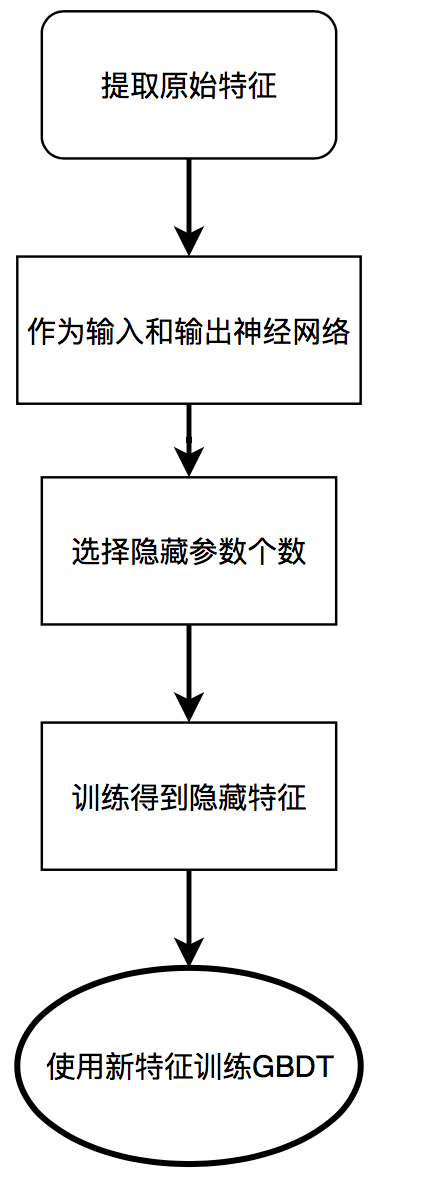
\includegraphics[width=0.4\textwidth]{chap3/auto-flow}
    \bicaption[fig:auto-flow]{自动编码器算法流程图}{自动编码器算法流程图}{Fig.}{Autoencoder Flowchart}
\end{figure}

\begin{algorithm}
    \caption{自动编码器人群预测算法}
    \label{algo:auto-algo}
    \begin{algorithmic}[1]
    \State Initial Data
    \For{$i = 1 \to N$}
        \State $F_{i,j} \gets LTE\_location(i,j), j=1,2,...,T$
        \State ${F'}_{i,j} \gets Autoencoder(F_{i,j}), j=1,2,...,T$
        \State $F_{i,j} \gets F_{i,j} + {F'}_{i,j}, j=1,2,...,T$
        \State $Train(F_{i,j}), j=1,2,...,T-k$
        \State $Y_i \gets Predict(F_{i,T+j}), j=1,2,...,k$
        \State $E_{i,T+j} \gets \frac{|Y_{i,T+j}-D_{i,T+j}|}{D_{i,T+j}}, j=1,2,...,k$
        \State $E_i \gets {\sqrt  {\sum _{{j=1}}^{k}E_{i,T+j}^{2} \over k}}$
    \EndFor
    \State $E \gets {\sum _{{i=1}}^{N}E_{i} \over N}$
    \State 
    \Return $E$
    \end{algorithmic}
\end{algorithm}

\section{本章小结}

在本章中我们详细分别介绍了基于拟合的人群密度预测算法,以及基于机器学习的人群密度预测算法。其中机器学习的预测算法,我们分别使用了基于GBDT和相邻区域特征的监督学习算法和基于自动编码器的无监督学习算法。在第四章节中我们将分别对这几种算法进行实验对比。 